%================================================================
\chapter{Introduction}
\chaptermark{Introduction} 
%================================================================

\section{The Abraham-Minkowski momentum}

There has been a recent resurgence of interest in understanding the electromagnetic momentum density in a dielectric medium. Two different forms of the momentum density were proposed by Minkowski and Abraham over 100 years ago.  Minkowski argued that the momentum density of an electromagnetic field in matter be of the form 
\begin{equation}
\mathbf{g}_{\mathrm{M}}=\mathbf{D}\times\mathbf{B}
\end{equation}
while Abraham held 
\begin{equation}
\mathbf{g}_{\mathrm{A}}=\frac{1}{c^2}\mathbf{E}\times\mathbf{H}
\end{equation}
The Abraham-Minkowski dilemma can be recast in terms of the photon momentum traveling through a dielectric medium.  The Abraham photon momentum is $\mathbf{p}_{\mathrm{A}} = \hbar\omega/n$ while the Minkowski photon momentum is $\mathbf{p}_{\mathrm{M}} = \hbar\omega n$, where $n$ is refractive index of the material. It is hard to believe that such a seemingly trivial problem has not been sorted out yet, but after 100 years, the correct form remains enigmatic. The difficulty lies in the fact that experiments have been done which apparently support both forms. Consider the following two gedanken experiments. In the first experiment suggested by Balazs \cite{balazs}, a photon travels through a slab of transparent material \ref{fig:Thought1}.

%***************************figure**********************
\begin{figure}[htp]
\includegraphics[width=1\columnwidth]{./Figures/ThoughtExperiment1.pdf}
\caption{A thought experiment which supports the Abraham representation of the photon momentum.  In (A) a photon travels towards a stationary dielectric block of refractive index $n$.  In (B) we assume the photon is completely transmitted with no reflection.  The velocity of the photon slows down as it travels through the dielectric material to $c/n$.  By invoking a conservation of mass-energy argument, it's easy to show that the momentum of the photon inside the material should be the Abraham momentum $\hbar\omega/n$ } 
\label{fig:Thought1}
\end{figure}
%*********************************************************

The total energy of the system before the photon enters the median is $E_{\mathrm{total}} = \hbar\omega +Mc^2$, where $M$ is the mass of the slab. While traveling through the block, the photon speed slows down to $c/n$ and therefore would take a time $t = Ln/c$ to transverse the slab, where L is the length of the slab. Upon exiting the slab, the photon would have traveled a shorter distance than it would have had it traveled in free space. This difference in distance is $L(n-1)$. By uniformity of center of mass-energy, the block must be displaced by some distance $\Delta z$ in the direction of propagation of the photon. The uniform motion of the center of mass-energy requires that
\begin{equation}
L(n-1)\hbar\omega = ∆zMc^22
\label{deltaz}
\end{equation}
If we then assume that the momentum acquired from the slab came from the momentum lost by the photon, we obtain
\begin{equation}
\mathbf{p}_{\mathrm{slab}}=M\frac{\Delta z}{Ln/c}
\label{uniform}
\end{equation}
Solving for $\Delta z$ in Eq.\ (\ref{deltaz}) and plugging this into Eq.\ (\ref{uniform}) yields
\begin{equation}
\mathbf{p}_{\mathrm{slab}}=\left(1-\frac{1}{n}\right)\frac{\hbar\omega}{c}
\end{equation}
By conservation of momentum, we know the total momentum is given simply by the initial momentum of the system
\begin{equation}
\mathbf{p}_{\mathrm{total}} = \frac{\hbar\omega}{c}
\end{equation}
We then set this equal to the final total momentum $\mathbf{p}_{\mathrm{slab}}+\mathbf{p}_{\mathrm{photon}}$, 
and solve for the final photon momentum inside the slab
\begin{equation}
\mathbf{p}_{\mathrm{photon}}=\frac{\hbar\omega}{cn}=\mathbf{p}_{\mathrm{A}}
\end{equation}
This leaves us with the Abraham momentum.  

For the second gedanken experiment \cite{barnett}, consider an atom of mass $m$ with a transition frequency of $\omega$ traveling through a median with an index of refraction $n$, at velocity $v$. Let as also assume that the atom is moving away from a light source emitting at an angular frequency $\omega_0$. 

%***************************figure**********************
\begin{figure}[htp]
\includegraphics[width=1\columnwidth]{./Figures/ThoughtExperiment2.pdf}
\caption{A thought experiment which supports the Minkowski representation of the photon momentum.  In (A) a photon of optical frequency $\omega_0$ interacts with an atom of mass $m$ and transition frequency $\omega$, which is traveling through dielectric slab refractive index $n$ with a velocity $\mathbf{v}$.  In (B) the atom can only absorb the photons of the beam if the transition frequency math the laser frequency in the atom's frame of reference. Since the atom is moving with velocity $\mathbf{v}$, the atom see's the laser frequency shifted to $\omega^{'}=\omega_0(1-n\mathbf{v}/c)$.  Through conservation of energy and momentum, one finds that the photon momentum must be the Minkowski momentum $\hbar\omega n$ } 
\label{fig:Thought1}
\end{figure}
%*********************************************************



The atom can absorb a photon if the doppler shifted frequency matches the transition frequency of the atom. In this case we require
\begin{equation}
\omega=\omega_0(1-\frac{n\mathbf{v}}{c})
\label{freq}
\end{equation}

By conservation of energy and momentum we would then have
\begin{eqnarray}
&&\frac{1}{2}mv^2_{\mathrm{final}}+\hbar\omega_0=\frac{1}{2}mv^2_{\mathrm{initial}}+\hbar\omega \\
&&mv_{\mathrm{final}}=mv_{\mathrm{initial}}+\mathbf{p}_{\mathrm{photon}}
\end{eqnarray}
Combining these two equations with Eq.\ (\ref{freq}) and solving for the photon momentum yields $\mathbf{p}_{\mathrm{photon}}=\hbar\omega n$, which is none other than the Minkowski momentum!  So what is exactly is going on here?  How can both answers be correct?

\vspace{5mm}

	This thesis is an attempt to explain this paradox and to better understand the work done by other physicists on the subject.

\vspace{5mm}


The importance of unraveling this mystery go beyond toy gedanken experiments. Knowledge of the momentum of light in a medium is of importance in interferometry using electromagnetic waves to manipulate atoms. Experiments involving high precision measurements of the photon recoil momentum are used to determine the fine structure constant \cite{spectroscopy} .  In 2005, David Pritchard's group at MIT set out to determine whether atoms in a Rubidium BEC,  subjected to an optical pulse, recoiled in accordance to Minkowski or Abraham \cite{ketterle}.  Figure (\ref{fig:ketterle}) shows the experiment in which a standing wave pulse is applied to a BEC cloud of Rubidium atoms. The momentum kick out-couples a small fraction of atoms which evolve at a different rate from the other atoms.  After a short delay, a second pulse recombines the atoms and their interference is observed. This two-pulse Ramsey interferometer revealed a momentum kick in accordance with the Minkowski form of the momentum of light $\mathbf{p}_{M}=\hbar\omega n $.  
%***************************figure**********************
\begin{figure}[htp]
\includegraphics[width=1\columnwidth]{./Figures/KetterleImage.pdf}
\caption{An experiment preformed by the David Pritchard and Wolfgang Ketterle group at MIT \cite{ketterle} in which they attempt to discern the momentum of light in a medium.  A standing wave pulse is applied to a Rubidium BEC which outcouples a portion of the atoms from the zero momentum state into the $2\hbar k$ momentum state.  These atoms are allowed to evolve in this seperate state for $600$ms before being recombined with the original zero momentum batch.  The interference pattern is then imaged to determine the momentum kick the atoms received. They conclude that the momentum kick is modified by the presence of the BEC itself, and show that the atoms receive an impulse of $2\hbar k n$ - consistent with Minkowski's prediction.} 
\label{fig:ketterle}
\end{figure}
%*********************************************************

On the other hand, the Peng and Leonhardt's group claim to have demonstarted that the momentum of light traveling through a liguid is of the Abraham form $\mathbf{p}_{A}=\hbar\omega/n$ \cite{leonhardt2}.
%***************************figure**********************
\begin{figure}[htp]
\centering
\includegraphics[width=100mm,scale=0.5]{./Figures/Leonhardt.pdf}
\caption{An experiment preformed by Ulf Leonhardt and Nan Peng's group \cite{leonhardt2} on the optical force of light acting on a liquid. By balancing the momentum from the incident, reflected, and transmitted light with the surface tension, they predict that an inward bulge in the liquid would be indicative of the Abraham momentum of light, while an outward bulge, the Minkowski momentum. Upon lasing the surface, they observed an inward bulge in the liquid which corroborates the Abraham representation.} 
\label{fig:sphere}
\end{figure}
%*********************************************************



In his famous review on relativity \cite{pauli}, Pauli pointed out that the Abraham momentum density $\mathbf{g}_{A}$ gives the same ponderomotive force on a stationary dielectric as the Minkowski momentum density $\mathbf{g}_{M}$ except for an extra term, which we shall call the R\"{o}ntgen momentum,
\begin{equation}
\mathbf{p}_{\mathrm{Ront}}= \frac{\partial}{\partial t} (\mathbf{d} \times \mathbf{B} ) .
\label{eq:Ront}
\end{equation}
However, Pauli noted that ``Because of the smallness of this term, it is hardly likely that an experiment could be devised for deciding in favour of one or the other of the two approaches''. That has not stopped people from trying, and the last 100 years have seen many studies devoted to identifying the correct form of electromagnetic momentum density $\mathbf{g}$, including recent theory and experiments  \cite{Gordon73,chiao,Loudon05,ketterle,feng,mansuripur,hinds09,barnett10}. In particular, Gordon has convincingly shown that when the Lorentz force is used to calculate the ponderomotive force on a nondispersive dielectric medium the result agrees with the Abraham form \cite{Gordon73}. The Lorentz force approach allows for a physical interpretation of the origin of the R\"{o}ntgen term which is due to the Lorentz force on the internal electric current in an oscillating dipole due to the magnetic field [Check]. Hinds and Barnett used the Lorentz force approach to study the simplest dielectric of all, a single atom, interacting with a travelling pulse of laser light \cite{hinds09}. The standard optical dipole force predicts that an atom will be attracted into a red-detuned pulse, but they showed that the extra R\"{o}ntgen term given in Eq.\ (\ref{eq:Ront}) produces a force of twice the magnitude and in the opposite direction to the dipole force so that the atom is \emph{repelled} from the pulse. The experiment with the greatest relevance to the present work is that by Campbell \emph{et al} \cite{ketterle} who measured the recoil momentum of atoms scattered out of a Bose-Einstein condensate by a pulse of standing-wave light, and found the Minkowski result $\mathbf{p}_M$. 

It appears that there is now a consensus that both the Abraham and the Minkowski forms can be correct, depending upon exactly what is measured \cite{Loudon05,barnett10}. An important step in resolving the Abraham-Minkowski puzzle was the realization that $\mathbf{p}_{M}$ and $\mathbf{p}_A$ are the photon momenta associated with the canonical and kinetic momentum of the atoms, respectively.  This link appears to have first been established by Loudon, Babiker, Baxter and Lembessis \cite{lembessis}. This  allows for a more intuitive understanding of the mechanism responsible for the different responses seen in experiments. In particular, it can be argued that the Abraham momentum is associated with centre-of-mass motion of a medium, whereas if the medium is capable of diffracting (as cold atoms can), the Minkowski momentum is more relevant because the momentum operator in quantum mechanics is associated with the canonical momentum (we shall see in this thesis that this guess is not really true since we use diffraction to obtain a result in agreement with Abraham...).  In this thesis we extend this line of investigation by considering the quantum phases acquired by atoms interacting with light rather than the classical forces. Inside a plane wave laser beam an atom will feel no classical dipole force and yet will acquire a quantum phase due to the R\"{o}ntgen interaction (it is straightforward to show that in the path-integral formulation of quantum mechanics the term given in Eq.\ (\ref{eq:Ront}) leads directly to the HMW phase). This line of inquiry leads us to connect the Abraham momentum density with the so called He-McKellar-Wilkens (HMW) phase. 

\newpage




%============================== 
\section{The HMW phase}
Geometric phases were first generalized by Berry in 1984.  The geometric phase is a measure of the failure of certain variables to return to their original values after cycling around a closed circuit in some parameter space.  The simplest example is a tangent vector moving along a circuit on a sphere as shown in Figure (\ref{fig:sphere}).  The tangent vector is forced not to rotate about the normal vector perpendicular to the surface - also known as parallel transport. If the tangent vector begins and ends at the north pole, it is found upon completing the cycle, that a rotation in the arrow's orientation has accumulated during transport process.

%***************************figure**********************
\begin{figure}[htp]
\centering
\includegraphics[width=100mm,scale=0.5]{./Figures/sphere.pdf}
\caption{Parallel transport of a tangent vector along the surface of a sphere is an example of a geometric phase shift. Image courtesy of \cite{sphere}.} 
\label{fig:sphere}
\end{figure}
%*********************************************************

Now suppose instead of the tangent vector, we are considering the basis vectors ${\ket{\chi_g(\mathbf{r})},\ket{\chi_e(\mathbf{r})}} $ describing the ground and excited states of a two level atom. We can write the state of the atom $\Psi$ in terms of this basis as
\begin{equation}
\ket{\Psi(\mathbf{r},t)}=\psi_g(\mathbf{r},t)\ket{\chi_g(\mathbf{r})}+\psi_e(\mathbf{r},t)\ket{\chi_e(\mathbf{r})}
\label{statevector1}
\end{equation}
The evolution of this state vector is determined by the Schr\"{o}dinger equation
\begin{equation}
i\hbar\frac{\partial}{\partial t}\ket{\Psi(\mathbf{r},t)}=\left(\frac{-\hbar^2\nabla^2}{2M}+V+U\right)\ket{\Psi(\mathbf{r},t)}
\label{stateschrodinger}
\end{equation}
Where $U$ is the atom-field coupling operator, and $V$ is the external potential. The form of these operators is not important for this discussion. Note that the spatial derivative originating from the canonical momentum operator $\mathbf{P}$ acts not only on the amplitudes $\psi_j$, but also on the basis vectors $\ket{\chi_j}$. Suppose now we are interested in a situation in which $\psi_e=0$. This for example occurs whenever we are interested in the interaction of an atom with an electromagnetic field which is far detuned from the atomic transition of the atom.  In other words, whenever an atom is interacting with an electromagnetic field which is not on resonance with the atoms transition frequency. Plugging in Eq.\ (\ref{statevector1}) into Eq.\ (\ref{stateschrodinger}) and taking the dot product with the ground state vector $\ket{\chi_g}$ yields
\begin{equation}
i\hbar\frac{\partial}{\partial t}=\left[\frac{\left(\mathbf{P}-\mathbf{A}\right)}{2M}+V+U_{g}+\phi(r)\right]\psi_i
\end{equation}
where $\mathbf{A}=i\hbar\braket{\chi_g,\nabla \chi_g}$ is the vector potential, $\phi=\frac{\hbar^2}{2M}\left|\braket{\chi_g,\nabla \chi_g}\right|^2$
is the scalar potential, and $U_g$ is the component of the coupling operator along $\ket{g}$. 

What is of interest of us is the appearance of the vector potential $\mathbf{A}$ which arose due to the spatial dependence of the basis vectors. In Section 3, we will show that if one then calculates the accumulated phase the atom acquires traveling along some path $\Gamma$, the presence the vector potential $\mathbf{A}$ gives rise to an extra phase, in addition to the traditional dynamic phase, given by 
\begin{equation}
e^{\frac{i}{\hbar}\int_{\Gamma} \mathbf{A}(\mathbf{r})\cdot d\mathbf{r}}
\end{equation}
This phase only depends on the path, and not on the interaction time - hence the name geometric phase. Dynamic phases on the other hand are induced by classical forces.  As such they are characterized by their dependence on the interaction time, and hence the velocity of the particle in question.  Additionally, the dynamic phase is independent of direction of propagation. Geometric phases however are direction propagation dependent, and do not depend on the interaction time, and by extension, independent of the particle velocity.  These characterizing features will be used in Section 3 in order to differentiate geometric and dynamic perturbations.

\vspace{5mm}

This thesis primarily explores one such geometric phase which arises in atomic physics - The He-McKellar-Wilkens (HMW) phase. 

\vspace{5mm}

The HMW phase is a topological quantum phase predicted by He and McKellar in 1993 \cite{mckellar93} and independently by Wilkens in 1994 \cite{wilkens94}. It is one of a family of four such phases that includes the Aharonov-Bohm (AB) \cite{aharanov59} and Aharonov-Casher (AC) \cite{aharanov84} phases that are all related by electromagnetic dualities  \cite{dowling99}. The AB phase arises when a charged particle moves in a region of space where there is a nonzero magnetic vector potential $\mathbf{A}$ and yet the magnetic field $\mathbf{B}= \nabla \times \mathbf{A}$ vanishes, as is the case outside a solenoid. There is no force acting on the particle and according to classical mechanics the particle is unaffected by the presence of the solenoid. However, in the quantum case the particle's wave function is affected. Any path encircling the solenoid acquires the phase 
\begin{equation}
\phi_{\mathrm{AB}}=(q/ \hbar) \oint \mathbf{A}(\mathbf{r}) \cdot d \mathbf r
\label{eq:phiAB}
\end{equation}
 which can be seen in the interference pattern between paths passing on different sides of the solenoid. The significance of the AB phase is generally taken to be that it can either be viewed as a manifestation of the physical reality of electromagnetic potentials or of the non locality of quantum mechanics \cite{vaidmann}.  The HMW phase \cite{mckellar93,wilkens94}
 \begin{equation}
 \phi_{\mathrm{HMW}} = \hbar^{-1} \oint [\mathbf{B}(\mathbf{r}) \times \mathbf {d}] \cdot d \mathbf r 
 \label{eq:phiHMW}
 \end{equation}
  is associated with a neutral quantum particle endowed with an electric dipole moment $\mathbf{d}$ moving in a closed circuit in a static magnetic field of strength $\mathbf{B}$. Like the AC phase $\phi_{\mathrm{AC}} = -(\hbar c^2)^{-1} \oint [\mathbf{E}(\mathbf{r}) \times \boldsymbol{\mu}] \cdot d \mathbf r $, where a magnetic moment $\boldsymbol{\mu}$ moves in a static electric field and experiences to first order in $v/c$ the motional magnetic field $\mathbf{B}_{\mathrm{mot}} = - \mathbf{v} \times \mathbf{E} /c^2$, the electric dipole in the HMW phase  experiences a motional electric field $\mathbf{E}_{\mathrm{mot}} = \mathbf{v} \times \mathbf{B}$ leading to the R\"{o}ntgen interaction \cite{wilkens94}. In order to obtain a finite HMW (or AC) phase the physical electromagnetic fields should not vanish everywhere on the circuit (unlike in the AB phase) and yet various configurations of the fields and polarization have been proposed \cite{mckellar93,wilkens94,dowling99,wei95} where no forces appear to act and yet the phase is finite.  Indeed, it has been shown that the HMW phase can be derived by considering the sum of the two AB phases acquired by the two charges forming the dipole \cite{wei95}. 
 %***************************figure**********************
\begin{figure}[htp]
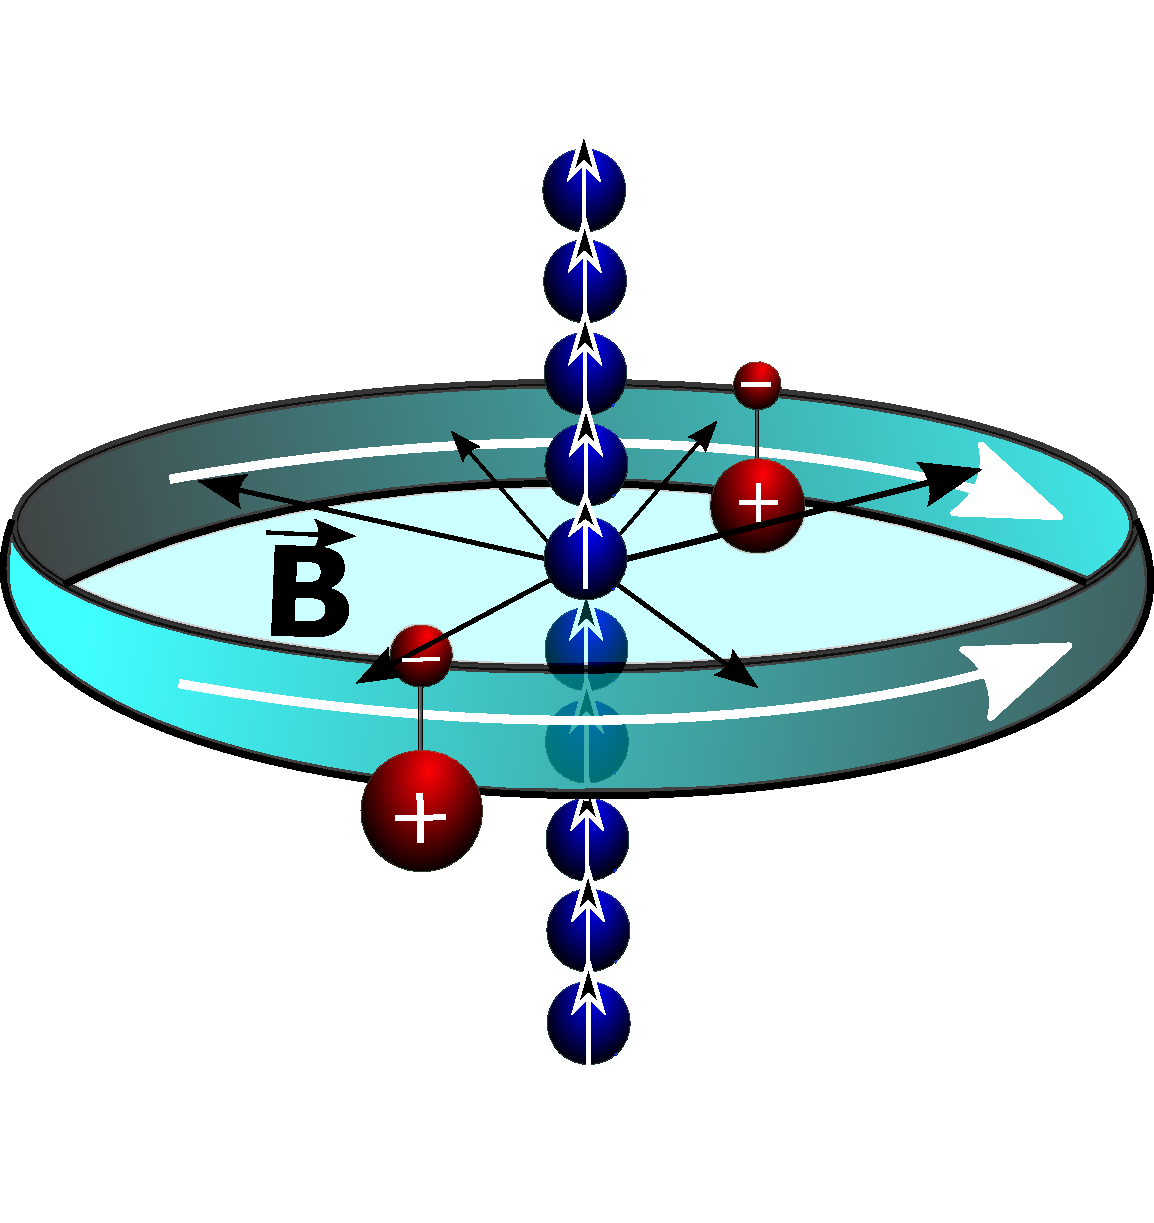
\includegraphics[width=150mm,scale=1]{./Figures/HMWnew.pdf}
\caption{The HWM phase $\phi_{\mathrm{HMW}} = \hbar^{-1} \oint [\mathbf{B}(\mathbf{r}) \times \mathbf {d}] \cdot d \mathbf r $ is analogous to the Aharonov-Casher phase with the magnetic dipole of the AC phase replaced with an electric dipole in the HMW arrangement, and the static radial electric field swapped with a static radial magnetic field. In this arrangement the radial magnetic field is always perpendicular to the dipole moment $\mathbf{d}$ providing a nonzero HWM phase without any classical forces acting on the atom.}
\label{fig:hmw}
\end{figure}
%*********************************************************  
%The AB phase for a circuit $\phi_{\mathrm{AB}}=(q/ \hbar) \oint \mathbf{A}(\mathbf{r}) \cdot d \mathbf r $  arises when a  particle with electric charge $q$ moves in a region of space where there is a nonzero magnetic vector potential $\mathbf{A}$ and yet the magnetic field $\mathbf{B}= \nabla \times \mathbf{A}$ vanishes, as is the case outside a solenoid.

Experimental confirmation of the AB \cite{chambers60,tonomura86,olariu85,peshkin89} and the AC  \cite{cimmino89,sangster93,zeiske95,gorlitz95,yanagimachi02} phases came quite quickly after the theoretical predictions and the experiments have continued to be refined over the years. The HMW phase was only recently detected in an experiment using lithium atoms in a Mach-Zehnder atom interferometer  \cite{vigue1,vigue2,vigue3,vigue4}. These latter experiments took care to establish that the phase was dispersionless (independent of velocity) and reversed sign when the direction of travel of the atoms was reversed. These properties are hallmarks of geometric phases (of which topological phases are a particular case) and are in contrast to dynamical phases. The latter originate from potentials (and thus forces) and depend on the time spent in the interferometer and hence inversely upon the speed of the atom. 


Both the HMW and the AC phases can be derived using the Feynman path integral approach which associates the phase $\int L dt$ with every path if we adopt the standard direct coupling Lagrangian $L$ supplemented by the motional fields
\begin{equation}
L=\frac{1}{2}m v^2 +  \mathbf{d} \cdot (\mathbf{E}+ \mathbf{v}\times \mathbf{B})+ \boldsymbol{\mu} \cdot (\mathbf{B}- \mathbf{v}\times \mathbf{E}/c^2)  
\label{eq:Lagrangian}
\end{equation}
where $m$ is the mass of the particle and $\mathbf{E}$ and $\mathbf{B}$ are specified in the laboratory frame.  Because we are interested in the optical regime where the $\mathbf{E}$ and $\mathbf{B}$ fields rapidly change sign, whereas $\mathbf{\mu}$ does not, we shall neglect the third term in Eq.\ (\ref{eq:Lagrangian}) because it vanishes when averaged over an optical cycle. The resulting Lagrangian can be compared to the standard \emph{minimal} coupling Lagrangian for a charged particle 
\begin{equation}
L=\frac{1}{2}m v^2 +  q  \mathbf{v} \cdot \mathbf{A} - q \phi
\end{equation}
where $\phi$ is the scalar potential. Comparing terms we can formally associate $\mathbf{B} \times \mathbf{d}$ with $q \mathbf {A}$ and $\mathbf{d} \cdot \mathbf{E}$ with $-q \phi$. In this way the HMW phase given in Eq.\ (\ref{eq:phiHMW}) follows directly from the AB phase given in Eq.\ (\ref{eq:phiAB}). Apart from the quantum HMW phase, these associations also suggest that we can treat the dipole as an effective charge interacting with the following effective fields
\begin{eqnarray}
\mathbf{B}_{\mathrm{eff}}  & \equiv & \nabla \times \mathbf{A}_{\mathrm{eff}} = \frac{1}{q} \nabla \times (\mathbf{B} \times \mathbf{d}) \label{eq:Beff} \\
\mathbf{E}_{\mathrm{eff}}  & \equiv & - \nabla \phi_{\mathrm{eff}} - \frac{\partial \mathbf{A}_{\mathrm{eff}} }{\partial t} = \frac{1}{q} \left[ \nabla (\mathbf{d} \cdot \mathbf{E}) - \frac{\partial}{\partial t} (\mathbf{B} \times \mathbf{d}) \right] . \label{eq:Eeff}
\end{eqnarray}
that account for (classical) electromagnetic forces on the dipole. In the linear response regime $\mathbf{d}=\alpha (\mathbf{E}+ \mathbf{v}\times \mathbf{B})$ \cite{wei95}, where $\alpha$ is the polarizability, and we can replace the second term in the Lagrangian by $(\alpha/2) (\mathbf{E}+ \mathbf{v}\times \mathbf{B})^2$. Following through the calculation we find that to lowest order in $v/c$ we can replace $\mathbf{B} \times \mathbf{d}$ by $\alpha (\mathbf{B} \times \mathbf{E})$ and $\mathbf{d} \cdot \mathbf{E}$ by $(\alpha/2) E^2$ in the Eqns.\ (\ref{eq:Beff}) and (\ref{eq:Eeff}). The terms depending on $\mathbf{B} \times \mathbf{E}$ are proportional to the local Poynting vector $\mathbf{S}=(\mathbf{E} \times \mathbf{B})/\mu_{0}$ of the optical field. In the plane wave laser beams we shall consider here, the Poynting vector has zero curl and so $\mathbf{B}_{\mathrm{eff}} =0$. The very interesting case of laser beams with non-zero orbital angular momentum such as Laguerre-Gauss beams that would give  $\mathbf{B}_{\mathrm{eff}} \neq 0$ will be considered elsewhere. We thus find that the force on the dipole in an optical field carrying zero orbital angular momentum is purely due to the effective electric field
\begin{equation}
\mathbf{F}=q \mathbf{E}_{\mathrm{eff}}= \nabla \left( \frac{\alpha}{2} E^2 \right)+\alpha \frac{\partial}{\partial t} (\mathbf{E} \times \mathbf{B}).
\end{equation}
The first term is the familiar induced dipole force that depends on the gradient of the intensity \cite{cohentannoudjibook}. The second term depends on the time-dependence of the Poynting vector. It is zero in static field configurations but gives a contribution, for example, when fields are turned on and off. Unlike the dipole force, it is nonconservative, a feature it shares with magnetic forces in general due to the form of the velocity dependence of the Lagrangian.
\newpage




%==============================
\section{This Thesis}

This thesis is organized into 6 sections.  In Section 2 I review the classical electromagnetic forces acting on an atom.  I show how the dipole and R\"{o}ntgen forces arise from the Lorentz force acting on the charges of an atom.  I then explore the energy-momentum tensor and show how the Abraham and Minkowski tensor representations differ through the R\"{o}ntgen force.  

In Section 3 I introduce the idea of atomic interferometry and review the Feynman path integral approach to calculating phases.  I next propose three different experimental arrangements capable of measuring the HMW phase through interferometric means.  The first is an optical Mach-Zehnder interferometer which has an optical beam running along the two arms of the inteferometer.  These traveling beams produce an HMW phase in the atoms as they travel along the length of the interferomter which is then measured via interference.  The second scheme is a Kapitza-Dirac interferometer which interferes a BEC with itself after splitting it into two groups and subjecting each group to an optical field.  The two groups acquire an HMW phase as a result and interfere with each other when finally recombined.  Finally, in the third setup, we consider a BEC in an optical ring trap irradiated by a Laguerre-Gaussian (LG) beam.  These LG beams carry angular momentum which interacts with the atoms traveling in the ring trap.  This interaction induces an HMW phase in the atoms which may then be measured by interfering these atoms with a control group.

In Section 4 I show how two different representation of the direct coupling Hamiltonian give rise to the Abraham or the Minkowski momentum.  The HMW and the AC phase arise naturally as a result of the unitary transformation linking the two representations.  

In Section 5, I approach the questions from the confines of an optical cavity.  Beginning with a toy model for a triple cavity system in which the central mirror is allowed to move, I show that the Abraham/Minkowski momentum representations arise as a result of bookkeeping.  If one assumes the energy of the electromagnetic field in matter is purely due to the photons themselves, then one obtains the Minkowski representation.  If on the other hand one accounts for the energy that goes into twisting and polarizing the atoms making up the medium, then one ends up with the Abraham representation.

Finally, in the last section, I review the main conclusions of this thesis and discuss future directions.

\newpage




%================================================================
